\documentclass[12pt, a4paper]{article}

% ── Packages ──────────────────────────────────────────────────────
\usepackage{fontspec}
\setmainfont{Arial}
\usepackage{amsmath, amssymb, amsthm}
\usepackage{mathtools}
\usepackage{enumitem}
\usepackage{tikz}
\usetikzlibrary{calc, positioning, arrows.meta, fit, patterns, decorations.pathreplacing}
\usepackage{geometry}
\geometry{margin=2.4cm}
\usepackage{xcolor}
\usepackage{tcolorbox}
\tcbuselibrary{theorems, skins, breakable}
\usepackage{booktabs}
\usepackage{hyperref}
\hypersetup{colorlinks=true, linkcolor=blue!60!black, urlcolor=blue!60!black}

\setlength{\parindent}{0pt}
\setlength{\parskip}{6pt}

% ── Colours ───────────────────────────────────────────────────────
\definecolor{setA}{RGB}{66, 133, 244}   % blue
\definecolor{setB}{RGB}{234, 67, 53}    % red
\definecolor{setC}{RGB}{251, 188, 4}    % yellow
\definecolor{theoryBg}{RGB}{232, 245, 253}
\definecolor{theoryFrame}{RGB}{66, 133, 244}
\definecolor{stmtBg}{RGB}{255, 243, 224}
\definecolor{stmtFrame}{RGB}{230, 126, 34}
\definecolor{ansBg}{RGB}{232, 250, 232}
\definecolor{ansFrame}{RGB}{39, 174, 96}

% ── Environments ──────────────────────────────────────────────────
\newtcolorbox{theorybox}[1][]{%
  colback=theoryBg, colframe=theoryFrame,
  fonttitle=\bfseries, title={\small Տեսական Ակնարկ. #1},
  breakable, enhanced, arc=2mm,
  left=5pt, right=5pt, top=5pt, bottom=5pt
}

\newtcolorbox{problembox}{%
  colback=stmtBg, colframe=stmtFrame,
  fonttitle=\bfseries, title={\small Խնդրի Պահանջ},
  breakable, enhanced, arc=2mm,
  left=5pt, right=5pt, top=5pt, bottom=5pt
}

\newtcolorbox{answerbox}{%
  colback=ansBg, colframe=ansFrame,
  arc=2mm, left=5pt, right=5pt, top=3pt, bottom=3pt
}

\newcommand{\Z}{\mathbb{Z}}
\newcommand{\R}{\mathbb{R}}
\newcommand{\N}{\mathbb{N}}
\newcommand{\powset}[1]{2^{#1}}
\newcommand{\comp}[1]{\overline{#1}}
\newcommand{\symdiff}{\mathbin{\triangle}}

% ── Title ─────────────────────────────────────────────────────────
\title{\textbf{Գործնական 7 — Տրոհումներ և ներառման-բացառման սկզբունքը}\\[4pt]
       \large Ընտրված խնդիրների լուծումներ\\[2pt]
       \normalsize Խնդիրներ 1, 7, 10, 12}
\author{Դիսկրետ Մաթեմատիկա — ԵՊՀ}
\date{}

\begin{document}
\maketitle
\tableofcontents
\newpage

% ══════════════════════════════════════════════════════════════════
\section{Խնդիր 1 — 5-էլեմենտանի բազմության տրոհումը 3 դասերի}
% ══════════════════════════════════════════════════════════════════

\begin{theorybox}[Երկրորդ սեռի Ստիռլինգի թվեր]
\textbf{Երկրորդ սեռի Ստիռլինգի թիվը}՝ $S(n,k)$-ն, հաշվում է $n$-տարրանի բազմության տրոհումների քանակը ճիշտ $k$ հատ ոչ դատարկ, զույգ առ զույգ չհատվող ենթաբազմությունների (որոնք կոչվում են \emph{դասեր} կամ \emph{բլոկներ})։

\medskip
\textbf{Անդրադարձ առնչություն՝}
\[
  S(n,k) = S(n-1,\, k-1) \;+\; k \cdot S(n-1,\, k),
  \qquad n \ge 1,\; 1 \le k \le n։
\]

\textbf{Մեկնաբանություն՝}\; Դիտարկենք $n$-րդ տարրը։
\begin{itemize}[nosep]
  \item \emph{$n$-ը միայնակ է իր դասում՝}\;
        մնացած $n-1$ տարրերը կազմում են $k-1$ դասեր
        $\;\longrightarrow\; S(n-1,\,k-1)$ եղանակ։
  \item \emph{$n$-ը միանում է գոյություն ունեցող $k$ դասերից մեկին՝}\;
        նախ տրոհում ենք մնացած $n-1$ տարրերը $k$ դասերի
        ($S(n-1,\,k)$ եղանակ), ապա ընտրում ենք, թե որ դասին է միանում $n$-ը ($k$ ընտրություն)
        $\;\longrightarrow\; k \cdot S(n-1,\,k)$ եղանակ։
\end{itemize}

\medskip
\textbf{Եզրային պայմաններ՝}\;
$S(n,1) = 1$,\; $S(n,n) = 1$,\; $S(n,0) = 0$, երբ $n \ge 1$։

\begin{center}
\begin{tikzpicture}[scale=0.8, font=\small]
  % Set partition visual: {1,4}, {2,5}, {3}
  \node[font=\bfseries] at (-2, 1) {Օրինակ՝ $S(5,3)$};
  
  \node (n1) at (0,1.5) {1};
  \node (n4) at (1,1.5) {4};
  \node[draw=setA, thick, rounded corners, fit=(n1)(n4), inner sep=2pt, label={below:\tiny $\{1,4\}$}] {};
  
  \node (n2) at (2.5,1.5) {2};
  \node (n5) at (3.5,1.5) {5};
  \node[draw=setB, thick, rounded corners, fit=(n2)(n5), inner sep=2pt, label={below:\tiny $\{2,5\}$}] {};
  
  \node (n3) at (5,1.5) {3};
  \node[draw=setC!80!black, thick, rounded corners, fit=(n3), inner sep=2pt, label={below:\tiny $\{3\}$}] {};
  
  \node at (2.5, 0.5) {Տրոհում 3 բլոկի};
\end{tikzpicture}
\end{center}

\begin{center}
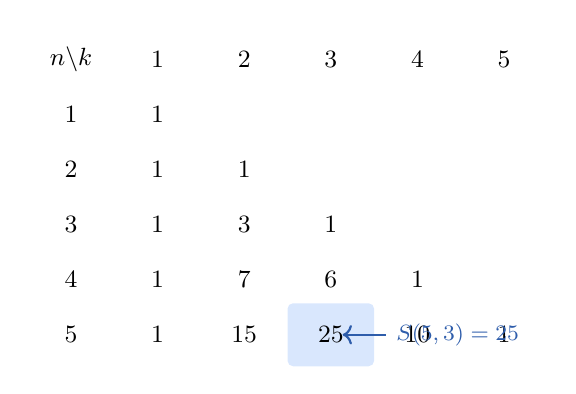
\begin{tikzpicture}[
  cell/.style={minimum width=1.1cm, minimum height=0.8cm, font=\small, anchor=center},
  header/.style={cell, font=\small\bfseries}
]
  % Header row
  \node[header] at (0, 0) {$n \backslash k$};
  \foreach \k [count=\i] in {1,2,3,4,5} {
    \node[header] at (\i*1.1, 0) {$\k$};
  }
  % Data rows
  \foreach \n/\vals [count=\row] in {
    1/{1},
    2/{1,1},
    3/{1,3,1},
    4/{1,7,6,1},
    5/{1,15,25,10,1}%
  } {
    \node[cell, font=\small\bfseries] at (0, -\row*0.7) {$\n$};
    \foreach \v [count=\col] in \vals {
      \ifnum\row=5
        \ifnum\col=3
          \node[cell, fill=setA!20, rounded corners=2pt] at (\col*1.1, -\row*0.7) {$\v$};
        \else
          \node[cell] at (\col*1.1, -\row*0.7) {$\v$};
        \fi
      \else
        \node[cell] at (\col*1.1, -\row*0.7) {$\v$};
      \fi
    }
  }
  % Highlight annotation
  \draw[->, thick, setA!70!black] (3.3+0.7, -3.5) -- (3.3+0.15, -3.5)
    node[right, pos=0, font=\footnotesize, setA!70!black] {$S(5,3)=25$};
\end{tikzpicture}
\end{center}
\end{theorybox}

\begin{problembox}
Քանի՞ եղանակով կարելի է $5$-տարրանի բազմությունը տրոհել $3$ ոչ դատարկ դասերի։
\end{problembox}

\subsection*{Լուծում}

Մեզ անհրաժեշտ է գտնել $S(5,3)$ Ստիռլինգի թիվը։ Օգտվելով անդրադարձ առնչությունից՝
\[
  S(5,3) = S(4,2) + 3 \cdot S(4,3)։
\]

\textbf{Հաշվում ենք $S(4,2)$-ը՝}
\[
  S(4,2) = S(3,1) + 2 \cdot S(3,2) = 1 + 2 \cdot 3 = 7։
\]

\textbf{Հաշվում ենք $S(4,3)$-ը՝}
\[
  S(4,3) = S(3,2) + 3 \cdot S(3,3) = 3 + 3 \cdot 1 = 6։
\]

\textbf{Վերջնական արդյունք՝}
\[
  S(5,3) = 7 + 3 \cdot 6 = 7 + 18 = 25։
\]

\textbf{Անկախ ստուգում։}\; Հաստատենք սա՝ դասակարգելով տրոհումները ըստ բլոկների չափերի (տրոհման կառուցվածք՝ $\{3,1,1\}$ և $\{2,2,1\}$)։

\textbf{Ստուգում բացահայտ թվարկմամբ։}\;
Դիցուք՝ բազմությունն է $\{a,b,c,d,e\}$։ 3 դասերի տրոհումը պետք է ունենա $\{3,1,1\}$ կամ $\{2,2,1\}$ կառուցվածքը (5-ի միակ տրոհումները 3 մասերի)։

\begin{itemize}[nosep]
  \item \textbf{Տիպ $\{3,1,1\}$՝}\;
        Ընտրում ենք 3-տարրանի բլոկը՝ $\binom{5}{3} = 10$ եղանակ։
        Մնացած 2 միատարր բազմությունները կազմում են չկարգավորված զույգ, որը տալիս է $1$ դասավորություն։
        Ընդամենը՝ $10$։
  \item \textbf{Տիպ $\{2,2,1\}$՝}\;
        Ընտրում ենք մեկ տարր պարունակող բլոկը՝ $\binom{5}{1} = 5$ եղանակ։
        Մնացած 4 տարրերը տրոհում ենք երկու զույգերի՝
        $\frac{1}{2!}\binom{4}{2} = 3$ եղանակ (բաժանում ենք $2!$-ի, քանի որ երկու զույգերը
        չկարգավորված են)։
        Ընդամենը՝ $5 \times 3 = 15$։
\end{itemize}

Ընդհանուր գումար՝ $10 + 15 = 25$։ \;\checkmark

\begin{answerbox}
\centering $S(5,3) = \boxed{25}$
\end{answerbox}

% ══════════════════════════════════════════════════════════════════
\newpage
\section{Խնդիր 7 — Բաժանելիությունը և Ներառման-բացառման սկզբունքը}
% ══════════════════════════════════════════════════════════════════

\begin{theorybox}[Ներառման-բացառման սկզբունք]
Վերջավոր բազմության (ունիվերսի) $A_1, A_2, \ldots, A_m$ ենթաբազմությունների համար՝
\[
  \biggl|\,\bigcup_{i=1}^{m} A_i\biggr|
  = \sum_{i} |A_i|
  - \sum_{i<j} |A_i \cap A_j|
  + \sum_{i<j<k} |A_i \cap A_j \cap A_k|
  - \cdots
\]

\begin{center}
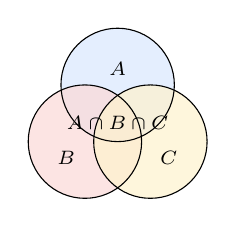
\begin{tikzpicture}[scale=0.6, font=\scriptsize]
  % 3-set Venn
  \coordinate (A) at (90:0.8);
  \coordinate (B) at (210:0.8);
  \coordinate (C) at (330:0.8);
  \fill[setA!20, opacity=0.7] (A) circle (1.2);
  \fill[setB!20, opacity=0.7] (B) circle (1.2);
  \fill[setC!20, opacity=0.7] (C) circle (1.2);
  \draw (A) circle (1.2) node[above] {$A$};
  \draw (B) circle (1.2) node[below left] {$B$};
  \draw (C) circle (1.2) node[below right] {$C$};
  \node at (0,0) {$A \cap B \cap C$};
\end{tikzpicture}
\end{center}

Հաշվելու համար այն տարրերը, որոնք չեն պատկանում $A_1, \ldots, A_m$ բազմություններից \textbf{ոչ մեկին}՝
\[
  \bigl|\comp{A_1} \cap \comp{A_2} \cap \cdots \cap \comp{A_m}\bigr|
  = |U| - \biggl|\,\bigcup_{i=1}^{m} A_i\biggr|։
\]

\medskip
\textbf{Կիրառությունը բաժանելիության խնդիրներում՝}\;
$\{1, 2, \ldots, N\}$ բազմության մեջ $d$-ի վրա բաժանվող ամբողջ թվերի քանակը
$\lfloor N/d \rfloor$ է։
Եթե $\gcd(d_1, d_2) = 1$, ապա միաժամանակ $d_1$-ի և $d_2$-ի վրա բաժանելիությունը համարժեք է $d_1 d_2$-ի վրա բաժանելիությանը։

\begin{center}
\begin{tikzpicture}[>=Stealth, font=\small, scale=0.85]
  \def\rr{1.6}
  \coordinate (cA) at (-0.65, 0);
  \coordinate (cB) at (0.65, 0);

  % Shade A only
  \begin{scope}
    \clip (cA) circle (\rr);
    \fill[setA!20] (-4,-4) rectangle (4,4);
  \end{scope}
  % Shade B only
  \begin{scope}
    \clip (cB) circle (\rr);
    \fill[setB!15] (-4,-4) rectangle (4,4);
  \end{scope}
  % Overlap
  \begin{scope}
    \clip (cA) circle (\rr);
    \clip (cB) circle (\rr);
    \fill[purple!20] (-4,-4) rectangle (4,4);
  \end{scope}

  \draw[thick, setA] (cA) circle (\rr);
  \draw[thick, setB] (cB) circle (\rr);

  \node[font=\footnotesize\bfseries, setA!70!black] at (-1.7, 1.1) {$A$};
  \node[font=\footnotesize\bfseries, setB!70!black] at (1.7, 1.1) {$B$};
Որոշում ենք ունիվերսալ բազմությունը (տիեզերքը) $S = 
  \node[font=\scriptsize] at (-1.4, 0.25) {$|A|-|A\!\cap\! B|$};
  \node[font=\scriptsize] at (0, -0.25) {$|A\!\cap\! B|$};
  \node[font=\scriptsize] at (1.4, 0.25) {$|B|-|A\!\cap\! B|$};

  \node[font=\footnotesize] at (0, -2.2) {$|A \cup B| = |A| + |B| - |A \cap B|$};
\end{tikzpicture}
\end{center}
\end{theorybox}

\begin{problembox}
$1$-ից $16500$ միջակայքում քանի՞ ամբողջ թիվ կա, որ չի բաժանվում $5$-ի, չի բաժանվում $3$-ի, բայց \textbf{բաժանվում է} $11$-ի վրա։
\end{problembox}

\subsection*{Լուծում}

\textbf{Քայլ 0. Ընտրում ենք ունիվերսը։}\; Ներառման-բացառման ցանկացած խնդրում առաջին քայլը \emph{ունիվերսի ընտրությունն է}։ Այստեղ մենք որպես $S$ վերցնում ենք $\{1, \ldots, 16500\}$ միջակայքի այն թվերը, որոնք բաժանվում են 11-ի։ Բոլոր հաշվարկները կատարվում են $S$-ի ներսում։

\medskip
Դիցուք $S$-ը $\{1, 2, \ldots, 16500\}$ հատվածի այն ամբողջ թվերի բազմությունն է, որոնք բաժանվում են $11$-ի։ Մենք ցանկանում ենք $S$-ից հեռացնել այն թվերը, որոնք բաժանվում են նաև $3$-ի կամ $5$-ի։

Սահմանենք՝
\begin{align*}
  A &= \{n \in S \mid 3 \mid n\}
      &&\text{(բաժանվում է և՛ 11-ի, և՛ 3-ի, այսինքն՝ 33-ի)}, \\
  B &= \{n \in S \mid 5 \mid n\}
      &&\text{(բաժանվում է և՛ 11-ի, և՛ 5-ի, այսինքն՝ 55-ի)}։
\end{align*}

Մենք փնտրում ենք $|S| - |A \cup B|$ արժեքը։

\textbf{Քայլ 1. Հաշվում ենք առանձին քանակները։}
\[
\renewcommand{\arraystretch}{1.3}
\begin{array}{rclcl}
  |S| &=& \lfloor 16500/11 \rfloor &=& 1500, \\
  |A| &=& \lfloor 16500/33 \rfloor &=& 500, \\
  |B| &=& \lfloor 16500/55 \rfloor &=& 300, \\
  |A \cap B| &=& \lfloor 16500/165 \rfloor &=& 100։
\end{array}
\]
Այստեղ $|A \cap B|$-ն հաշվում է $\text{lcm}(33,55) = 165$-ի վրա բաժանվող թվերը։

\textbf{Քայլ 2. Կիրառում ենք ներառման-բացառման սկզբունքը։}
\[
  |A \cup B| = |A| + |B| - |A \cap B| = 500 + 300 - 100 = 700։
\]

\textbf{Քայլ 3. Հանում ենք։}
\[
  |S \setminus (A \cup B)| = |S| - |A \cup B| = 1500 - 700 = 800։
\]

\begin{center}
\begin{tikzpicture}[>=Stealth, font=\small, scale=0.9]
  % Universe = S (div by 11)
  \draw[thick, gray, rounded corners=8pt, fill=gray!5]
    (-3.2, -2.0) rectangle (3.2, 2.2);
  \node[gray, font=\footnotesize\bfseries] at (2.5, 1.9) {$S\;(1500)$};

  \def\rr{1.2}
  \coordinate (cA) at (-0.5, 0);
  \coordinate (cB) at (0.5, 0);

  \fill[setA!20] (cA) circle (\rr);
  \fill[setB!15] (cB) circle (\rr);
  \begin{scope}
    \clip (cA) circle (\rr);
    \fill[purple!25] (cB) circle (\rr);
  \end{scope}

  \draw[thick, setA] (cA) circle (\rr);
  \draw[thick, setB] (cB) circle (\rr);

  \node[font=\footnotesize\bfseries, setA!70!black] at (-1.6, 0.8) {$A$};
  \node[font=\footnotesize\bfseries, setB!70!black] at (1.6, 0.8) {$B$};

  \node[font=\scriptsize] at (-1.1, 0) {$400$};
  \node[font=\scriptsize] at (0, 0) {$100$};
  \node[font=\scriptsize] at (1.1, 0) {$200$};

  \node[font=\footnotesize, ansFrame!80!black] at (-2.4, -1.3) {\textbf{800}};
  \draw[->, thick, ansFrame!70!black] (-2.4, -1.1) -- (-2.4, -0.2);
  \node[font=\scriptsize, gray] at (-2.4, -1.6) {պատ․};
\end{tikzpicture}
\end{center}

\begin{answerbox}
\centering $\boxed{800}$ թիվ 1-ից 16500 միջակայքում բաժանվում է 11-ի,
բայց ոչ 3-ի և ոչ էլ 5-ի։
\end{answerbox}

% ══════════════════════════════════════════════════════════════════
\newpage
\section{Խնդիր 10 — Եռանկյուններ եռանկյունաձև ցանցում}
% ══════════════════════════════════════════════════════════════════

\begin{theorybox}[Եռանկյունների հաշվումը եռանկյունաձև ցանցում]
Երբ հավասարակողմ եռանկյան յուրաքանչյուր կողմ բաժանվում է $n$ հավասար հատվածների, և բաժանման կետերը միացվում են կողմերին զուգահեռ գծերով, առաջանում է $n$ կողմով \textbf{եռանկյունաձև ցանց}։

\medskip
Ցանցը պարունակում է երկու տիպի եռանկյուններ, որոնց կողմերը զուգահեռ են սկզբնական եռանկյան կողմերին՝

\begin{enumerate}[nosep]
  \item \textbf{Դեպի վեր ուղղված} ($s$ կողմով, $1 \le s \le n$)՝
        $U(n,s) = \binom{n-s+2}{2}$։
  \item \textbf{Դեպի վար ուղղված} ($s$ կողմով, $1 \le s \le \lfloor n/2 \rfloor$)՝
        $D(n,s) = \binom{n-2s+2}{2}$։
\end{enumerate}

\begin{center}
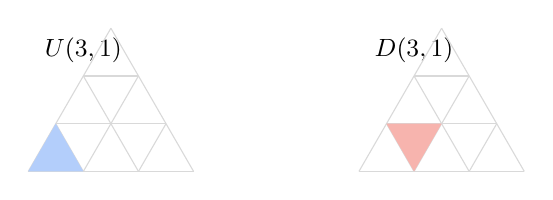
\begin{tikzpicture}[scale=0.7, font=\small]
  % Visual explosion of U/D
  % Base U triangle
  \begin{scope}[xshift=-3cm]
    \node[anchor=south] at (1, 1.8) {$U(3,1)$};
    \foreach \i in {0,...,3} \draw[gray!30] (\i/2, {\i*sqrt(3)/2}) -- (3 - \i/2, {\i*sqrt(3)/2});
    \foreach \i in {0,...,3} \draw[gray!30] (\i, 0) -- (\i/2, {\i*sqrt(3)/2});
    \foreach \i in {0,...,3} \draw[gray!30] (\i, 0) -- ({(3+\i)/2}, {(3-\i)*sqrt(3)/2});
    \fill[setA!40] (0,0) -- (1,0) -- (0.5,{sqrt(3)/2}) -- cycle;
  \end{scope}

  % Base D triangle
  \begin{scope}[xshift=3cm]
    \node[anchor=south] at (1, 1.8) {$D(3,1)$};
    \foreach \i in {0,...,3} \draw[gray!30] (\i/2, {\i*sqrt(3)/2}) -- (3 - \i/2, {\i*sqrt(3)/2});
    \foreach \i in {0,...,3} \draw[gray!30] (\i, 0) -- (\i/2, {\i*sqrt(3)/2});
    \foreach \i in {0,...,3} \draw[gray!30] (\i, 0) -- ({(3+\i)/2}, {(3-\i)*sqrt(3)/2});
    \fill[setB!40] (0.5,{sqrt(3)/2}) -- (1.5,{sqrt(3)/2}) -- (1,0) -- cycle;
  \end{scope}
\end{tikzpicture}
\end{center}

\begin{center}
\begin{tikzpicture}[scale=0.7, font=\small]
  % Small grid n=4 for illustration
  \def\n{4}
  % Draw grid lines
  \foreach \i in {0,...,\n} {
    % horizontal-ish lines (parallel to base)
    \draw[gray!50] (\i/2, {\i*sqrt(3)/2}) -- (\n - \i/2, {\i*sqrt(3)/2});
    % left-leaning lines
    \draw[gray!50] (\i, 0) -- (\i/2, {\i*sqrt(3)/2});
    % right-leaning lines
    \draw[gray!50] (\i, 0) -- ({(\n+\i)/2}, {(\n-\i)*sqrt(3)/2});
  }
  % Outer triangle
  \draw[thick] (0,0) -- (\n, 0) -- (\n/2, {\n*sqrt(3)/2}) -- cycle;

  % Highlight an upward triangle of side 2 (blue)
  \fill[setA!25, opacity=0.6] (0,0) -- (2,0) -- (1, {sqrt(3)}) -- cycle;
  \draw[thick, setA] (0,0) -- (2,0) -- (1, {sqrt(3)}) -- cycle;
  \node[font=\scriptsize, setA!70!black] at (1, 0.5) {$s\!=\!2$};

  % Highlight a downward triangle of side 1 (red)
  \fill[setB!25, opacity=0.6] (1.5, {sqrt(3)/2}) -- (2, 0) -- (2.5, {sqrt(3)/2}) -- cycle;
  \draw[thick, setB] (1.5, {sqrt(3)/2}) -- (2, 0) -- (2.5, {sqrt(3)/2}) -- cycle;

  % Labels
  \node[font=\footnotesize] at (2, -0.9) {Ցանց $n=4$-ով};
  \node[font=\scriptsize, setA!70!black] at (-1.8, 1.5) {դեպի վեր};
  \draw[->, setA!70!black, thin] (-1.0, 1.35) -- (0.4, 0.8);
  \node[font=\scriptsize, setB!70!black] at (4.6, 1.5) {դեպի վար};
  \draw[->, setB!70!black, thin] (4.0, 1.3) -- (2.3, 0.45);
\end{tikzpicture}
\end{center}
\end{theorybox}

\begin{problembox}
$ABC$ եռանկյան յուրաքանչյուր կողմը բաժանված է $8$ հավասար հատվածների։
Բաժանման կետերով անցնող և կողմերին զուգահեռ տարված ուղիղները կազմում են եռանկյունաձև ցանց։
Քանի՞ եռանկյուն կարելի է կազմել այս ցանցի կետերով, որոնց կողմերը զուգահեռ են $ABC$-ի կողմերին։
\end{problembox}

\subsection*{Լուծում}

Ունենք եռանկյունաձև ցանց $n = 8$ պարամետրով։ Մենք հաշվում ենք դեպի վեր և դեպի վար ուղղված եռանկյունները առանձին։

\textbf{Ի՞նչ ենք հաշվում։}\; «$s$ կողմով դեպի վեր եռանկյունը» այն եռանկյունն է, որն ունի նույն կողմնորոշումը, ինչ արտաքին եռանկյունը, և որի կողմը ընդգրկում է $s$ ցանցային միավոր։ «$s$ կողմով դեպի վար եռանկյունը» շրջված է։ Երկու տիպերն էլ պետք է ունենան արտաքին եռանկյանը զուգահեռ կողմեր։

\textbf{$s$ կողմով դեպի վեր եռանկյուններ ($1 \le s \le 8$)՝}
\[
  U(8,s) = \frac{(8-s+1)(8-s+2)}{2} = \binom{10-s}{2}։
\]

\begin{center}
\renewcommand{\arraystretch}{1.3}
\begin{tabular}{c|cccccccc|c}
\toprule
$s$ & 1 & 2 & 3 & 4 & 5 & 6 & 7 & 8 & Գումար \\
\midrule
$U(8,s)$ & 36 & 28 & 21 & 15 & 10 & 6 & 3 & 1 & \textbf{120} \\
\bottomrule
\end{tabular}
\end{center}

\[
  \sum_{s=1}^{8} U(8,s) = 36 + 28 + 21 + 15 + 10 + 6 + 3 + 1 = 120.
\]

\textbf{$s$ կողմով դեպի վար եռանկյուններ
($1 \le s \le \lfloor 8/2 \rfloor = 4$)՝}
\[
  D(8,s) = \frac{(8-2s+1)(8-2s+2)}{2} = \binom{10-2s}{2}։
\]

\begin{center}
\renewcommand{\arraystretch}{1.3}
\begin{tabular}{c|cccc|c}
\toprule
$s$ & 1 & 2 & 3 & 4 & Գումար \\
\midrule
$D(8,s)$ & 28 & 15 & 6 & 1 & \textbf{50} \\
\bottomrule
\end{tabular}
\end{center}

\[
  \sum_{s=1}^{4} D(8,s) = 28 + 15 + 6 + 1 = 50.
\]

\textbf{Ընդհանուր գումար՝}
\[
  120 + 50 = 170։
\]

\begin{center}
\begin{tikzpicture}[scale=0.38, font=\small]
  % Draw the n=8 grid
  \def\n{8}
  \foreach \i in {0,...,\n} {
    \draw[gray!40] (\i/2, {\i*sqrt(3)/2}) -- (\n - \i/2, {\i*sqrt(3)/2});
    \draw[gray!40] (\i, 0) -- (\i/2, {\i*sqrt(3)/2});
    \draw[gray!40] (\i, 0) -- ({(\n+\i)/2}, {(\n-\i)*sqrt(3)/2});
  }
  \draw[very thick] (0,0) -- (\n, 0) -- (\n/2, {\n*sqrt(3)/2}) -- cycle;

  % Example upward triangle of side 3 (blue)
  \fill[setA!20, opacity=0.5] (0.5, {sqrt(3)/2}) -- (3.5, {sqrt(3)/2})
    -- (2, {4*sqrt(3)/2}) -- cycle;
  \draw[thick, setA] (0.5, {sqrt(3)/2}) -- (3.5, {sqrt(3)/2})
    -- (2, {4*sqrt(3)/2}) -- cycle;

  % Example downward triangle of side 2 (red)
  \fill[setB!20, opacity=0.5] (3, {2*sqrt(3)/2}) -- (5, {2*sqrt(3)/2})
    -- (4, {0*sqrt(3)/2+0}) -- cycle;
  \draw[thick, setB] (3, {2*sqrt(3)/2}) -- (5, {2*sqrt(3)/2})
    -- (4, 0) -- cycle;

  \node[font=\footnotesize\bfseries] at (4, -1.2) {Ցանց $n = 8$-ով};
\end{tikzpicture}
\end{center}

\begin{answerbox}
\centering $ABC$-ի կողմերին զուգահեռ եռանկյունների ընդհանուր քանակը
$\boxed{170}$ է\; (120 դեպի վեր $+$ 50 դեպի վար)։
\end{answerbox}

% ══════════════════════════════════════════════════════════════════
\newpage
\section{Խնդիր 12 — Սահմանափակմամբ ամբողջ լուծումներ}
% ══════════════════════════════════════════════════════════════════

\begin{theorybox}[Ամբողջ լուծումների հաշվումը վերին սահմաններով]
$y_1 + y_2 + \cdots + y_r = n$ հավասարման ոչ բացասական ամբողջ լուծումները հաշվելու համար՝ $y_i \le u_i$ սահմանափակումներով.

\begin{enumerate}[nosep]
  \item \textbf{Առանց վերին սահմանների՝}\;
        Լուծումների քանակը $\binom{n+r-1}{r-1}$ է («աստղերի և գծիկների» մեթոդ)։
  \item \textbf{Հանում ենք խախտումները}՝ օգտագործելով ներառման-բացառման սկզբունքը։
        Դիցուք $A_i$-ն այն լուծումների բազմությունն է, որտեղ $y_i > u_i$։
        Տեղադրելով $z_i = y_i - (u_i + 1) \ge 0$՝ $|A_i|$ քանակը
        դառնում է առանց սահմանափակման խնդիր՝ նվազեցված գումարով։
  \item \textbf{Հատումներ՝}\;
        $|A_i \cap A_j|$-ի համար տեղադրում ենք և՛ $z_i = y_i - (u_i+1)$,
        և՛ $z_j = y_j - (u_j+1)$։
        Եթե մնացած գումարը բացասական է, ապա լուծումների քանակը $0$ է։
\end{enumerate}

\medskip
\textbf{Բանաձև՝}
\[
  \text{պատասխան} = \sum_{S \subseteq \{1,\ldots,r\}} (-1)^{|S|}
  \binom{n - \sum_{i \in S}(u_i+1) + r - 1}{r-1},
\]
որտեղ բինոմիալ գործակցի բացասական վերին անդամով դեպքերը հավասար են $0$-ի։
\end{theorybox}

\begin{problembox}
Գտնել ամբողջ լուծումների քանակը հետևյալ համակարգի համար՝
\[
  x_1 + x_2 + x_3 = 40, \qquad
  4 \le x_1 \le 15, \quad
  9 \le x_2 \le 18, \quad
  5 \le x_3 \le 16։
\]
\end{problembox}

\subsection*{Լուծում}

\textbf{Քայլ 1. Փոփոխականների տեղաշարժ ստորին սահմանները հեռացնելու համար։}

Նշանակենք $y_1 = x_1 - 4$,\; $y_2 = x_2 - 9$,\; $y_3 = x_3 - 5$։
Այդ դեպքում՝
\[, \quad
        z_1 + y_2 + y_3 = 10\text{։}
  &\quad |A_1| &= \binom{12}{2} = 66\text{։} \\
  A_2 &:\; y_2 \ge 10. \quad
        \text{Տեղադրենք } z_2 = y_2 - 10 \ge 0, \quad
        y_1 + z_2 + y_3 = 12\text{։}
  &\quad |A_2| &= \binom{14}{2} = 91\text{։} \\
  A_3 &:\; y_3 \ge 12. \quad
        \text{Տեղադրենք } z_3 = y_3 - 12 \ge 0, \quad
        y_1 + y_2 + z_3 = 10\text{։}
  &\quad |A_3| &= \binom{12}{2} = 66\text{։}

\textbf{Քայլ 3. Սահմանում ենք խախտման բազմությունները և կիրառում ներառման-բացառման սկզբունքը։}

Դիցուք $A_i$-ն այն լուծումների բազմությունն է, որտեղ $y_i$-ն գերազանցում է իր վերին սահմանը.
\begin{align*}
  A_1 &:\; y_1 \ge 12. \quad
        \text{Տեղադրենք } z_1 = y_1 - 12 \ge 0;\;
        z_1 + y_2 + y_3 = 10.
  &\quad |A_1| &= \binom{12}{2} = 66. \\
  A_2 &:\; y_2 \ge 10. \quad
        \text{Տեղադրենք } z_2 = y_2 - 10 \ge 0;\;
        y_1 + z_2 + y_3 = 12.
  &\quad |A_2| &= \binom{14}{2} = 91. \\
  A_3 &:\; y_3 \ge 12. \quad
        \text{Տեղադրենք } z_3 = y_3 - 12 \ge 0;\;
        y_1 + y_2 + z_3 = 10.
  &\quad |A_3| &= \binom{12}{2} = 66:
\end{align*}

\textbf{Քայլ 4. Զույգ առ զույգ հատումներ։}

$A_1 \cap A_2$: $y_1 \ge 12,\; y_2 \ge 10$.
Մնացած գումարը՝ $22 - 12 - 10 = 0$։
\quad $|A_1 \cap A_2| = \binom{2}{2} = 1$։

$A_1 \cap A_3$: $y_1 \ge 12,\; y_3 \ge 12$.
Մնացած գումարը՝ $22 - 12 - 12 = -2 < 0$։
\quad $|A_1 \cap A_3| = 0$։
Բացասական մնացորդային գումարը նշանակում է, որ համակարգը անհնարին է. ոչ բացասական փոփոխականների գումարը չի կարող լինել բացասական, ուստի լուծումների քանակը $0$ է։

$A_2 \cap A_3$: $y_2 \ge 10,\; y_3 \ge 12$.
Մնացած գումարը՝ $22 - 10 - 12 = 0$։
\quad $|A_2 \cap A_3| = \binom{2}{2} = 1$։

\textbf{Քայլ 5. Եռակի հատում։}
\[
  A_1 \cap A_2 \cap A_3:\; y_1 \ge 12,\; y_2 \ge 10,\; y_3 \ge 12.
  \quad \text{Գումարը } \ge 34 > 22։ \quad |A_1 \cap A_2 \cap A_3| = 0։
\]

\textbf{Քայլ 6. Միավորում՝ ըստ ներառման-բացառման սկզբունքի։}
\begin{align*}
  |A_1 \cup A_2 \cup A_3|
  &= (66 + 91 + 66) - (1 + 0 + 1) + 0 \\
  &= 223 - 2 = 221։
\end{align*}

\textbf{Վերջնական հաշվարկ՝}
\[
  276 - 221 = 55։
\]

\begin{center}
\begin{tikzpicture}[>=Stealth, font=\small, scale=0.85]
  \def\rr{1.3}
  \coordinate (cA) at (90:0.55);
  \coordinate (cB) at (210:0.55);
  \coordinate (cC) at (330:0.55);

  \fill[setA!15] (cA) circle (\rr);
  \fill[setB!12] (cB) circle (\rr);
  \fill[setC!12] (cC) circle (\rr);

  % Pairwise overlaps
  \begin{scope}
    \clip (cA) circle (\rr);
    \fill[purple!20] (cB) circle (\rr);
  \end{scope}
  \begin{scope}
    \clip (cB) circle (\rr);
    \fill[orange!20] (cC) circle (\rr);
  \end{scope}

  \draw[thick, setA] (cA) circle (\rr);
  \draw[thick, setB] (cB) circle (\rr);
  \draw[thick, setC] (cC) circle (\rr);

  \node[font=\footnotesize\bfseries, setA!70!black] at (90:2.1) {$A_1\;(66)$};
  \node[font=\footnotesize\bfseries, setB!70!black] at (210:2.1) {$A_2\;(91)$};
  \node[font=\footnotesize\bfseries, setC!80!black] at (330:2.1) {$A_3\;(66)$};

  \node[font=\tiny] at (150:0.85) {$1$};
  \node[font=\tiny, gray] at (30:0.85) {$0$};
  \node[font=\tiny] at (270:0.85) {$1$};
  \node[font=\tiny, gray] at (0:0) {$0$};

  \node[font=\footnotesize] at (0, -2.5)
    {$|A_1 \cup A_2 \cup A_3| = 221$};
  \node[font=\footnotesize\bfseries, ansFrame!80!black] at (0, -3.2)
    {Պատասխան՝ $276 - 221 = 55$};
\end{tikzpicture}
\end{center}

\begin{answerbox}
\centering Ամբողջ լուծումների քանակն է՝ $\boxed{55}$։
\end{answerbox}

\end{document}